\documentclass[14pt, a4paper]{article}

\usepackage[T2A]{fontenc}
\usepackage[utf8]{inputenc}
\usepackage[english, russian]{babel}

\usepackage{amsmath}
\usepackage{float}
\usepackage{graphicx}
\graphicspath{{./images/}}

\begin{document}
    \thispagestyle{empty}

    \begin{center}
        Министерство науки и высшего образования Российской Федерации

        Федеральное государственно автономное образовательное учреждение высшего образования

        <<Омский государственный технический университет>>

        \vspace{1cm}
        Факультет информационных технологий и компьютерных систем

        Кафедра <<Прикладная математика и фундаметральная информатика>>

        \vspace{3cm}
        \textbf{Расчётно-графическая работа}

        по дисциплине <<Дополнительные главы математического анализа>>
    \end{center}
    
    \vspace{3cm}
    \begin{flushright}    
        \begin{tabular}{ r r }
            Студента & Курпенова Куата Ибраимовича \\
            \cline{2-2}
            & \tiny{фамилия, имя, отчество полностью} \\

            Курс & 2, группа ФИТ-212 \\
            \cline{2-2}
            Направление & 02.03.02 Прикладная математика \\
            \cline{2-2}
            & и фундаментальная информатика \\
            \cline{2-2}
            & \tiny{код, наименование} \\

            Руководитель & доц., канд. физ.-мат. наук \\
            \cline{2-2}
            & \tiny{должность, ученая степень, звание} \\
            & Девятерикова М. В. \\
            \cline{2-2}
            & \tiny{фамилия, инициалы} \\

            Выполнил & \\
            \cline{2-2}
            & \tiny{дата, подпись студента(ки)} \\

            Проверил & \\
            \cline{2-2}
            & \tiny{дата, подпись руководителя} \\

        \end{tabular}
    \end{flushright}
    
    \vspace*{\fill}
    \begin{center}
        Омск 2022
    \end{center}

    \newpage

    \section*{Задание 1}

    Решить двойной интеграл с помощью MATLAB:

    \[ \iint_D{\frac{1}{(\sqrt{x + y}){(1 + x + y)}^3}} \]
    \[ 0 \leq x \leq 1, 0 \leq y \leq 1 - x \]

    \subsection*{Решение}

    \begin{figure}[H]
        \centering
        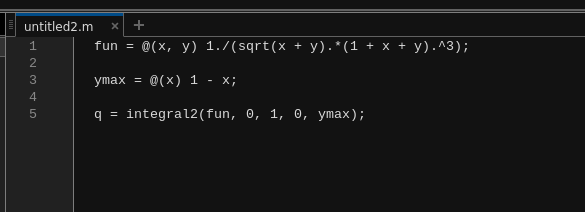
\includegraphics[width=\textwidth]{images/solution_integral.png}
        \caption{Код программы для решения двойного интеграла}
    \end{figure}

    \subsection*{Результат}

    \begin{figure}[H]
        \centering
        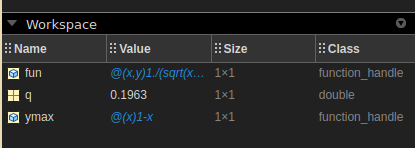
\includegraphics[width=\textwidth]{images/result_integral.png}
        \caption{Результат работы программы расчёта интеграла}
    \end{figure}

    \subsection*{Ответ}

    $\iint_D { \frac{ 1 } { (\sqrt{x + y}) { (1 + x + y) }^3 }} \approx 0.1963$

    \newpage
    
    \section*{Задание 2}

    Проверить ряд на сходимость при помощи MATLAB:

    \[ \sum_{n=1}^{\infty} \frac{5^{2n}}{(3n - 5)!} \]
    
    \subsection*{Решение}

    Решение будет сводиться к исследованию интеграла через признак Даламбера.

    \begin{figure}[H]
        \centering
        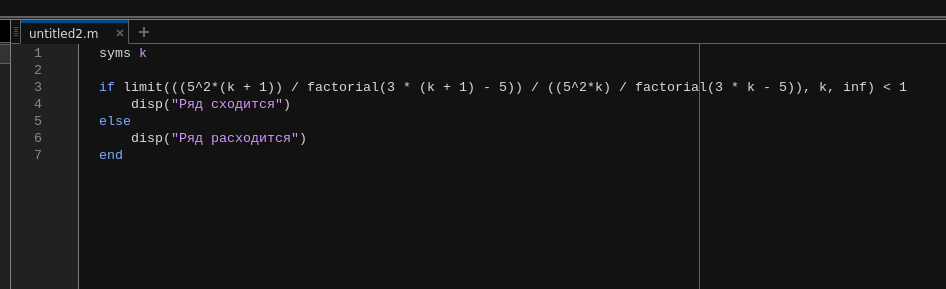
\includegraphics[width=\textwidth]{images/solution_row.png}
        \caption{Код программы для проверки ряда на сходимость}
    \end{figure}

    \subsection*{Результат}

    \begin{figure}[H]
        \centering
        
\includegraphics[width=\textwidth]{images/result_row.png}
        \caption{Результат работы программы проверки ряда на сходимость}
    \end{figure}

    \subsection*{Ответ}

    $\sum_{n=1}^{\infty} \frac{5^{2n}}{(3n - 5)!}$ - ряд сходится по признаку Даламбера.

\end{document}
